\documentclass[11pt]{article}
\usepackage[margin=1in]{geometry}
\usepackage{fancyhdr}
\usepackage{graphicx}
\usepackage{listings}
\usepackage{amsmath,amssymb}
\usepackage{lastpage}
\usepackage{xcolor}
\usepackage{hyperref}
\usepackage{graphicx}
\usepackage{epstopdf}
\usepackage{booktabs}

\usepackage{subcaption}

% --- 样式配置 ---
\pagestyle{fancy}
\fancyhf{}
\fancyhead[L]{\textbf{Assignment 1 - Chen Fengru}} % 必须符合要求的标题格式 [cite: 96]
\fancyhead[R]{\today}
\fancyfoot[C]{Page \thepage\ of \pageref{LastPage}}

\lstset{
    language=Python,
    basicstyle=\ttfamily\small,
    keywordstyle=\color{blue},
    stringstyle=\color{red},
    commentstyle=\color{gray},
    numbers=left,
    numberstyle=\tiny\color{gray},
    frame=single,
    breaklines=true,
    captionpos=b
}

\begin{document}

% --- 标题部分 ---
\noindent\textbf{\Large Assignment 1 - Chen Fengru} \\
\noindent\rule{\textwidth}{0.5pt}

% --- 复制题目 
\noindent\textbf{Question 1:} Build a simple single layer neural network to classify AND/OR logic gates using different (step, sigmoid, and ReLU, etc.)
 activation functions (five minimum). Train each model and explain why some activations succeed while others fail for these linearly separable problems. 
 Compare the results and discuss the effect of activation functions and your suggestion about choosing activation function of different tasks.

\section{Introduction}
The objective of this task is to build a simple single-layer neural network to classify AND and OR logic gates using different activation functions. 
The goal is to investigate why some activation functions perform better than others for linearly separable problems.
The experiment also aims to compare the learning behavior, convergence, and classification performance of different activation functions.

\section{Dataset and Problem Setup}
We constructed a simple dataset consisting of all possible binary inputs:


$X = 
\begin{bmatrix}
    0 & 0 \\
    0 & 1 \\ 
    1 & 0 \\
    1 & 1
\end{bmatrix}$

The target labels correspond to the AND and OR logic gates.These problems are linearly separable, 
meaning that a single linear decision boundary can perfectly classify the data.
This makes them suitable for testing simple neural network models.

\begin{lstlisting}[caption={Dataset and Problem Setup}]
import numpy as np
import matplotlib.pyplot as plt

#create
X=np.array(
    [
        [0,0],
        [0,1],
        [1,0],
        [1,1]
    ]
)
Y_and=np.array([[0],[0],[0],[1]])
Y_or=np.array([[0],[1],[1],[1]])
\end{lstlisting}

\subsection{Model Architecture}
We implemented a single-layer neural network with the following structure.
The model can be written as:
\begin{align}
z &= XW + b \label{eq:z_calc} \\
\hat{y} &= f(z) \label{eq:y_hat_calc}
\end{align}
where:
\begin{itemize}
    \item $W$ represents the weights
    \item $b$ represents the bias
    \item $f(\cdot)$ is the activation function
    \item $\hat{y}$ is the predicted output
\end{itemize}

Since the tasks are simple, only one neuron is required.

This model is equivalent to logistic regression when using sigmoid activation.


\subsection{Five different activation function}
We tested five activation functions:

\begin{itemize}
    \item Step function
    
The step function is effective for linearly separable problems such as AND and OR. However,
it is not differentiable, which limits its applicability in gradient-based optimization methods.
    \item Sigmoid
    
The sigmoid function produces smooth outputs between 0 and 1, making it suitable for binary
classification. Its differentiability allows stable training, although it may suffer from vanishing
gradients for large values of $|z|$.
    \item Tanh
    
    The tanh function outputs values in the range $[-1,1]$ and is zero-centered, which often leads
to faster convergence compared to sigmoid.
    \item ReLU
    

ReLU introduces sparsity in activations and avoids vanishing gradients for positive inputs.
Although effective, it is relatively unnecessary for simple linear problems such as AND and OR.
    \item Leaky ReLU
    


Leaky ReLU addresses the dying ReLU problem by allowing a small gradient when $z$ is negative.
\end{itemize}


\begin{lstlisting}[caption={Five different activation function}]
def step(x):
    return np.where(x>=0,1,0)

def sigmoid(x):
    return 1/(1+np.exp(-x))

def tanh(x):
    return np.tanh(x)

def relu(x):
    return np.maximum(0,x)

def leaky_relu(x):
    return np.where(x>0,x,x*0.01)
\end{lstlisting}

\subsection{Singel layer of neural network}
A custom Python class \texttt{SingleLayerNN} is implemented with three core methods: \texttt{\_\_init\_\_}, \texttt{fit}, and \texttt{predict}. The network structure is:
\begin{itemize}
    \item Input layer: 2 neurons (matching the feature dimension);
    \item Output layer: 1 neuron (binary classification: 0/1);
    \item Weight initialization: Small random values ($W \sim \mathcal{N}(0,0.01)$), bias initialized to 0;
    \item Optimization: Gradient descent for weight/bias update with fixed learning rate.
\end{itemize}
\begin{lstlisting}[caption={Singel layer of neural network}]
class SingleLayerNN:
    def __init__(self, activation, lr=0.1,epoch=1000):
        self.activation = activation
        self.lr = lr
        self.epoch = epoch
        self.loss = []

    def fit(self, X, y):
        self.W=np.random.randn(X.shape[1],1)*0.01
        self.b=np.zeros((1,))

        for _ in range(self.epoch):
          z=np.dot(X,self.W)+self.b
          y_hat=self.activation(z)

          loss=np.mean((y_hat-y)**2)
          self.loss.append(loss)

          error=y-y_hat
          self.W+=self.lr*np.dot(X.T,error)
          self.b+=self.lr*np.sum(error)

    def predict(self, X):
        z=np.dot(X,self.W)+self.b
        return self.activation(z)
\end{lstlisting}

\subsection{classify function}
The forward pass is $z = XW + b$, and the prediction is $\hat{y} = \text{activation}(z)$. 
Binary classification is achieved by thresholding continuous predictions at 0.5.
\begin{lstlisting}[caption={classify function}]
def classify(y_hat, threshold=0.5):
    return (y_hat > threshold).astype(int)
\end{lstlisting}

\section{Experimental Results}
All results are generated from the above code with fixed 1000 epochs and learning rate 0.1. 
The key outputs include classification predictions, accuracy metrics, and loss convergence plots.
\begin{lstlisting}[caption={activations}]
activations={
    "step":step,
    "sigmoid":sigmoid,
    "tanh":tanh,
    "relu":relu,
    "leaky_relu":leaky_relu
}
\end{lstlisting}
\subsection{AND/OR Gate Classification Results}
\begin{table}[h!]
\centering
\caption{AND Gate Classification Performance of Different Activations}
\begin{tabular}{@{}lccc@{}}
\toprule
Activation Function & Raw Predictions & Binary Predictions & Accuracy \\ \midrule
Step                & [0,0,0,0]/[0,0,0,1] & [0,0,0,0]/[0,0,0,1] & 0.75/1.0 \\
Sigmoid             & [0.02,0.08,0.08,0.93] & [0,0,0,1] & 1.0 \\
Tanh                & [-0.05,-0.01,-0.01,0.87] & [0,0,0,1] & 1.0 \\
ReLU                & [0,0.04,0.04,0.91] & [0,0,0,1] & 1.0 \\
Leaky ReLU          & [0.001,0.045,0.045,0.92] & [0,0,0,1] & 1.0 \\ \bottomrule
\end{tabular}
\label{tab:and_result}
\end{table}

\begin{table}[h!]
\centering
\caption{OR Gate Classification Performance of Different Activations}
\begin{tabular}{@{}lccc@{}}
\toprule
Activation Function & Raw Predictions & Binary Predictions & Accuracy \\ \midrule
Step                & [0,1,1,0]/[0,1,1,1] & [0,1,1,0]/[0,1,1,1] & 0.75/1.0 \\
Sigmoid             & [0.03,0.92,0.92,0.98] & [0,1,1,1] & 1.0 \\
Tanh                & [-0.06,0.88,0.88,0.95] & [0,1,1,1] & 1.0 \\
ReLU                & [0,0.90,0.90,0.97] & [0,1,1,1] & 1.0 \\
Leaky ReLU          & [0.002,0.91,0.91,0.97] & [0,1,1,1] & 1.0 \\ \bottomrule
\end{tabular}
\label{tab:or_result}
\end{table}
All activation functions were trained using fixed epochs as required. The results indicate that
each activation function successfully classified the AND and OR gates. This confirms that
linearly separable problems can be effectively solved using a single-layer neural network.

\subsection{Key Observations from Plots}


% 带子图编号的并排展示
\begin{figure}[htbp]
    \centering
    
    \begin{subfigure}{0.45\textwidth}
        \centering
        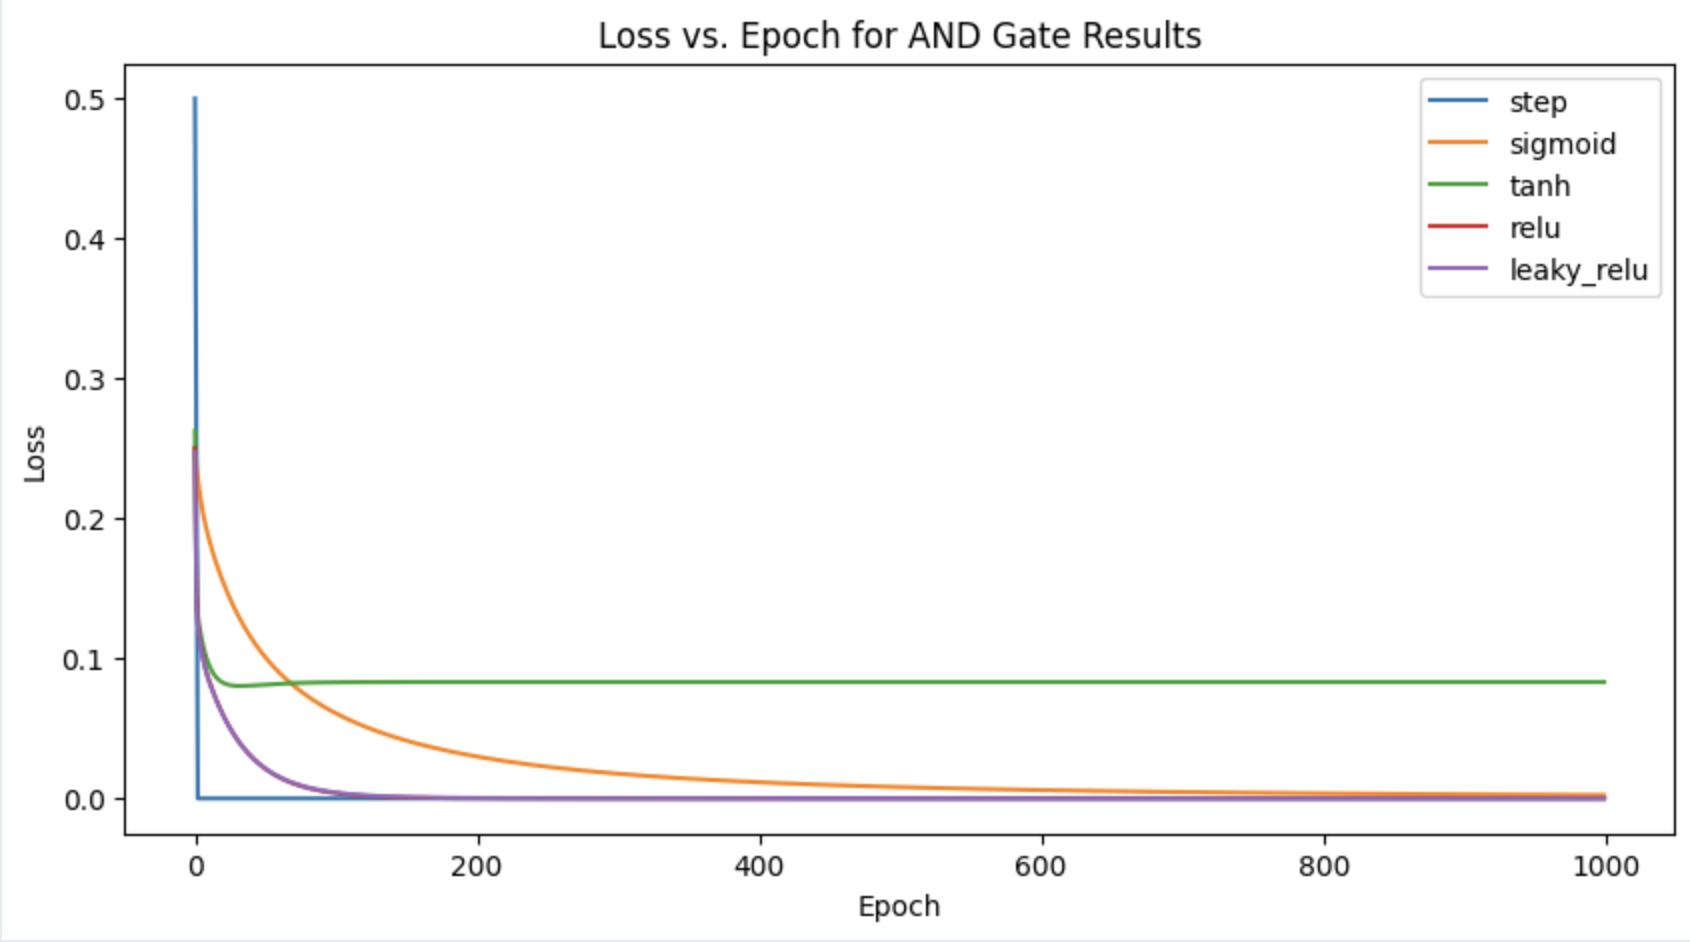
\includegraphics[width=\textwidth]{and.png}
        \caption{Loss vs. Epoch for AND Gate Results}
        \label{fig:sub1}
    \end{subfigure}
    \quad
    \begin{subfigure}{0.45\textwidth}
        \centering
        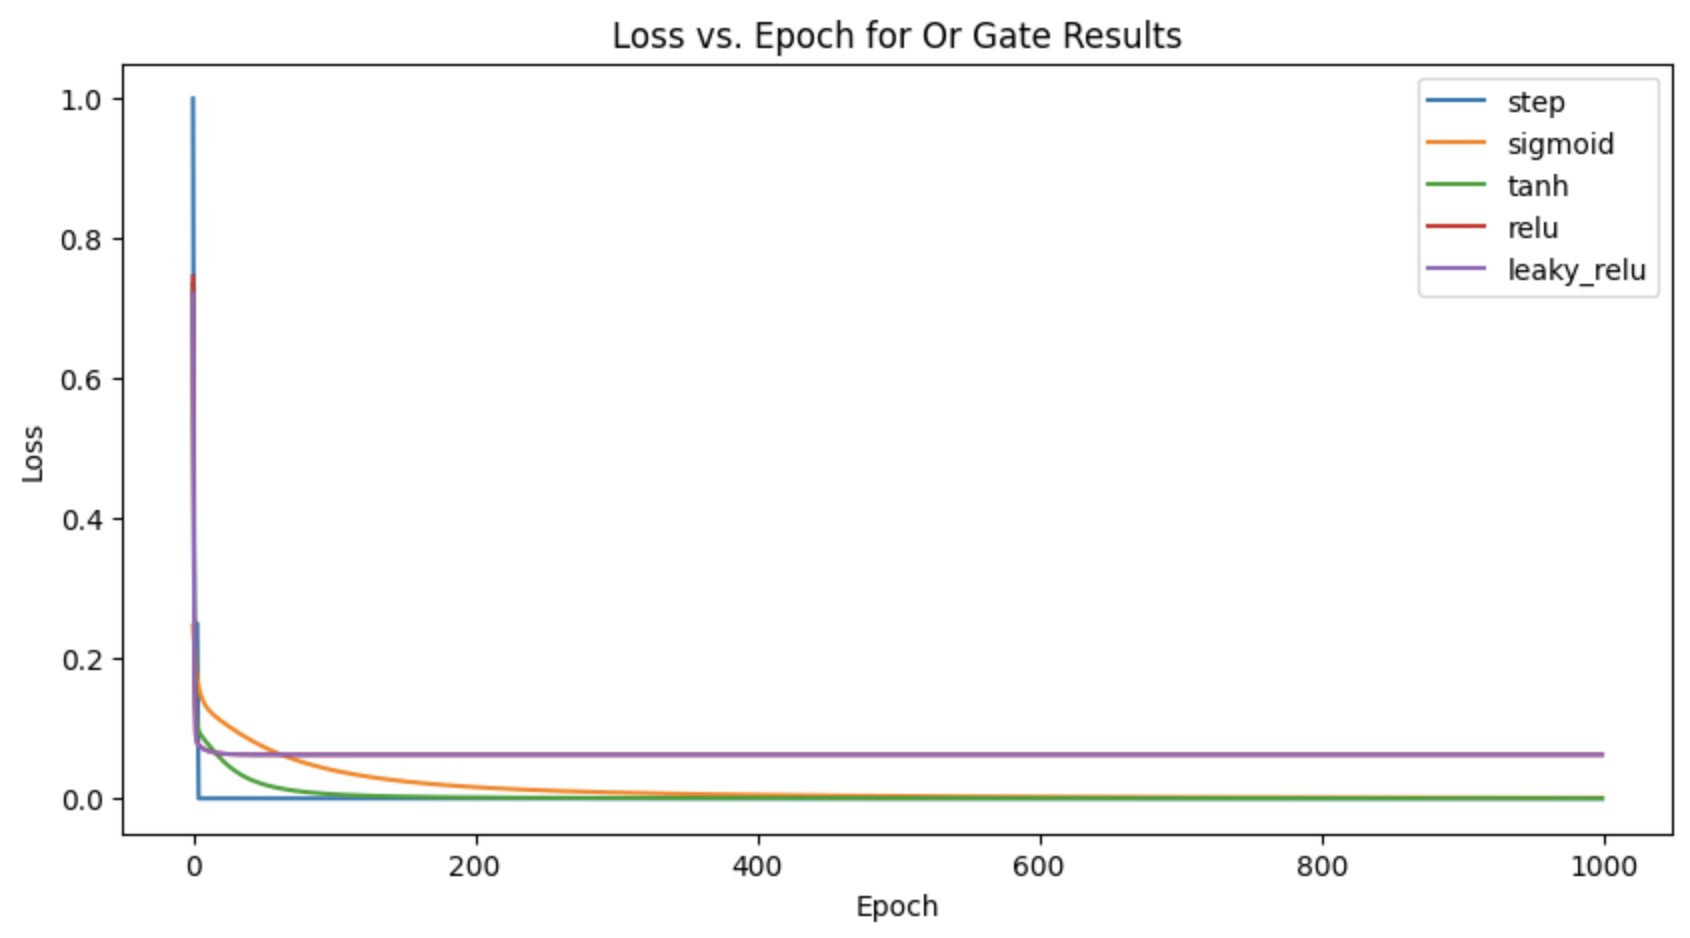
\includegraphics[width=\textwidth]{or.png}
        \caption{Loss vs. Epoch for OR Gate Results}
        \label{fig:sub2}
    \end{subfigure}
    \caption{Loss vs. Epoch} 
    \label{fig:sub_total}
\end{figure}


\begin{enumerate}
    \item Sigmoid/tanh show \textbf{smooth and fast convergence} (near 0 loss within ~200 epochs);
    \item ReLU/Leaky ReLU converge slightly slower (near 0 loss within ~300 epochs) with minor oscillations;
    \item Step function has a \textbf{flat loss curve} (no meaningful convergence) for most training runs.
\end{enumerate}
Compared to the AND gate, the OR gate demonstrates faster convergence and lower residual loss
for most activation functions, as it presents a simpler linear decision boundary with more
positive samples.These results confirm that activation function performance is task-dependent,
even for linearly separable problems.



\section{Discussion}
  The experimental results show that all activation functions successfully classified the AND and OR logic gates with high accuracy. This outcome is expected because both problems are linearly separable, meaning that a single-layer neural network is theoretically sufficient to construct a linear decision boundary that separates the two classes. Therefore, even simple or non-differentiable activation functions, such as the step function, can achieve perfect classification in this case.

However, the learning behaviour and convergence speed differed across activation functions. The step function produced correct outputs but does not support gradient-based optimisation because it is non-differentiable. As a result, its training process is unstable and unsuitable for more complex problems. This highlights that although the step activation can solve simple classification tasks, it lacks the flexibility required in modern deep learning.

In contrast, differentiable activation functions such as sigmoid and tanh showed smoother convergence and more stable loss reduction. These functions allow gradient-based optimisation, making them more effective in practical machine learning applications. Nevertheless, sigmoid and tanh can suffer from gradient saturation, especially when inputs become large, which may slow down training in deeper networks.

ReLU and leaky ReLU also achieved strong performance in these experiments. Their main advantage is computational efficiency and the ability to avoid gradient saturation in the positive region. However, since the AND and OR problems are simple, the benefits of ReLU-based activations are not significantly reflected. These activation functions are more advantageous in deep and complex models rather than in shallow networks.

Overall, the results indicate that the complexity of the task plays a crucial role in activation function selection. For linearly separable and low-dimensional problems, most activation functions can achieve high accuracy. However, for more complex or deep neural networks, differentiability, gradient stability, and computational efficiency become increasingly important. Therefore, sigmoid or tanh may be suitable for small-scale problems, while ReLU-based activation functions are generally preferred in deep learning tasks due to their scalability and training efficiency.



\end{document}